\documentclass[a4paper,10pt,french]{article}

\usepackage[
    xetex,
    margin=2cm,
    headheight=0.4cm,
    headsep=0.8cm,
    footskip=1.2cm,
    nomarginpar,
]{geometry}

\usepackage{xcolor}
\definecolor{linkcolor}{rgb}{0, 0, 0.6}

\usepackage[
    xetex,
    unicode=true,
    pdfstartview=FitV,
    colorlinks=true,
    citecolor=linkcolor,
    linkcolor=linkcolor,
    urlcolor=linkcolor,
    hyperindex=true,
]{hyperref}

\usepackage{amsmath} % Est-ce qu’on va vraiment s’en servir ?

\usepackage[version=4]{mhchem}

\usepackage{siunitx}
\sisetup{
    number-unit-product = \,,
    inter-unit-product = \ensuremath{{}\cdot{}},
    separate-uncertainty = true,
    multi-part-units = single,
    range-phrase = \text{ -- },
    range-units = single
}

\usepackage{enumitem}
\setitemize{itemsep = 1ex}

\usepackage{cleveref}

\usepackage{fontspec}
\usepackage{babel}

\usepackage{graphicx}
\graphicspath{{figures/}}
\usepackage{subcaption}

\usepackage{titling}
\title{Stage d’observation à l’IRAM}
\author{Maximilien Franco, Mélissa Menu, Bruno Pagani \& Jan Vatant--d’Ollone}
\date{14 au 19 mars 2016}

\hypersetup{
    pdfauthor={\theauthor},
    pdftitle={M2 AAIS – Stage en Observatoire},
    pdfsubject={\thetitle},
    pdfkeywords={M2 AAIS, Observatoire, IRAM, Grenade, 30m}
}

\usepackage{fancyhdr}
\pagestyle{fancy}
\fancyhead[L]{\scriptsize\textsc{\thetitle}}
\fancyhead[R]{\scriptsize\textsc{\theauthor}}
\fancyfoot[C]{\thepage}

\newcommand{\setup}{\textit{setup}}
\newcommand{\troismm}{\SI{3}{\milli\meter}}
\newcommand{\unmm}{\SI{1}{\milli\meter}}
\newcommand{\GHz}{\si{\giga\hertz}}

\begin{document}

\pagenumbering{roman}

% Pour faciliter la mise en forme des pages de garde, on supprime l’indentation
% automatique en début de paragraphe
\setlength{\parindent}{0pt}

% Pas d’en-tête ni de pied pour la première page
\thispagestyle{empty}


\includegraphics[height=2cm]{logo_insu.jpg} \hfill

\includegraphics[height=2cm]{logo_obspm.jpg} \hfill

\includegraphics[height=2cm]{logo_iap.jpg} \hfill

\includegraphics[height=2cm]{logo_psl.png}

\vspace{0.5cm}

\noindent
\begin{minipage}{.5\textwidth}
    \textsc{Master Astronomie, Astrophysique} \\
    \textsc{et Ingénierie Spatiale} \\
    \textit{M2R – Observatoire de Paris}
\end{minipage}%
\begin{minipage}{.5\textwidth}
    \begin{flushright}
        Stage d’Observation 2015--2016 \\
        Maximilien \textsc{Franco}, Mélissa \textsc{Menu}, \\
        Bruno \textsc{Pagani} \& Jan \textsc{Vatant--d’Ollone}
    \end{flushright}
\end{minipage}


\begin{center}

    \vspace{1.5cm}

    \rule[11pt]{5cm}{0.5pt}

    \textbf{\huge \thetitle}

    \rule{5cm}{0.5pt}

    \vspace{1.5cm}

    \parbox{15cm}{\textbf{Résumé} :
        La compréhension des processus conduisant à la formation d’étoiles est
        une question majeure de l’astrophysique. Les observations de la
        cinématique et de la composition des nuages proto-stellaires peuvent
        apporter des éléments déterminants dans l’étude de ces mécanismes. Nous
        proposons ici une présentation succincte et les premiers résultats des
        observations du nuage L1251B réalisées à l’Institut de Radio-Astronomie
        Millimétrique (IRAM) de Grenade à l’aide du télescope de
        \SI{30}{\meter} dans le cadre du stage d’observation du M2 AAIS. Un des
        objectifs centraux de cette étude était la réalisation de cartes
        d’émission de \ce{^12CO}, \ce{^13CO} et \ce{C^18O} ainsi qu’une
        caractérisation des espèces chimiques présentes dans ce milieu et la
        détermination précise des vitesses d’éjection spécifiques pour chaque
        composant.
    }

    \vspace{0.5cm}

    \parbox{15cm}{
        \textbf{Mots-clefs} : \it M2 AAIS – Observatoire – Grenade – IRAM – 30m
    }

    \vspace{0.5cm}

    \parbox{15cm}{
        Stage encadré par :

        \textbf{Anaëlle Maury} \\
        \href{mailto:anaelle.maury@cea.fr}{\tt anaelle.maury@cea.fr} / tél. (+33) 1 69 08 36 61 \\
        CEA/DRF/IRFU/SAp/LFEMI – Bât. 709 – Bureau 131 \\
        Service d’Astrophysique (SAp – UMR7158 Astrophysique, Instrumentation et Modélisation) \\
        Laboratoire de Formation des Etoiles et du Milieu Interstellaire (LFEMI) \\
        \url{http://irfu.cea.fr/Sap/}

        \textit{%
            CEA – Centre d’Études de Saclay \\
            Orme des Merisiers \\
            91191 Gif-sur-Yvette CEDEX
        }
    }

    \vspace{0.5cm}

    \hfill 
\includegraphics[height=2.5cm]{logo_cea.pdf} \hfill 
\includegraphics[height=2.5cm]{logo_irfu.png} \hfill 
\includegraphics[height=2.5cm]{logo_aim.jpg} \hfill \null \\
    \vspace{0.5cm}
    \hfill 
\includegraphics[height=2.5cm]{logo_iram.png} \hfill 
\includegraphics[height=2.5cm]{logo_upd.png} \hfill \null \\

\end{center}

\vfill
\hfill \thedate

\newpage

\thispagestyle{empty}

\section*{Remerciements}

Nous remercions tous le personnel de l’IRAM pour son accueil chaleureux, que ce
soit les opérateurs, techniciens en tous genre ou les cuisinières, ainsi que
les différents chercheurs (Joshua \textsc{Greenslade}, Alvaro \textsc{Hacar} et
Gabriel \textsc{Paubert}) présents sur place pour les différents échanges que
nous avons eus avec eux. Nous souhaitons remercier également l’ensemble des
personnes ayant participé à l’organisation de ce stage d’observation, que ce
soit à l’IRAM, l’Observatoire, au CEA ou l’Université Paris–Diderot, et
particulièrement à celles qui ont permis la mise en place de ce partenariat il
y a maintenant quelques années.

Enfin, un grand merci à Anaëlle Maury pour son investissement et son
accompagnement tout au long de ce stage, du voyage et de sa préparation, ainsi
que pour les nombreuses et riches discussions que nous avons eues avec elle.

\tableofcontents

\newpage

\pagenumbering{arabic}

\setlength{\parindent}{16pt}
\setlength{\parskip}{1ex}

\section{Avant-propos}

Le temps de télescope étant précieux, nous nous sommes préparés plusieurs mois
avant le début du stage afin de profiter au mieux du temps d’observation qui
nous était accordé. Nous avons effectué un certain nombre de séances de
préparation en amont. Il s’agissait de prendre connaissance avec le sujet et
les objets, les observations souhaitées, le télescope et son fonctionnement…

Les observations avaient pour objectif de mieux comprendre les phénomènes ayant
lieu dans la zone de formation stellaire L1251B. La cartographie effectuée
durant cette semaine permettra de confronter certaines théories, notamment sur
le rôle des jets dans la cinématique et les turbulences au sein des amas
proto-stellaires.

TODO: Un peu plus de blabla sur les sources, leur intérêt. Inclure des figures
envoyées par Anaelle.

TODO: Du blabla sur les fréquences d’intérêt, pourquoi elles le sont.

\begin{table}
    \centering
    \caption[]{Liste des fréquences des principales transitions des molécules attendues}
    \label{frequence_transition}
    \begin{tabular}{ccc}
        \hline
        \hline
        Molécule & Transition & Fréquence (\GHz) \\
        \hline
        \ce{H^13CO+}   &(1-0)       & \num{ 86.754285} \\
        \ce{HCN}       &(1-0)       & \num{ 88.631847} \\
        \ce{HCO+}      &(1-0)       & \num{ 89.188523} \\
        \ce{N2H+}      &(1-0)       & \num{ 93.176258} \\
        \ce{CH3OH}     &(2-1)       & \num{ 96.741377} \\
        \ce{CS}        &(2-1)       & \num{ 97.980968} \\
        \ce{C^18O}     &(1-0)       & \num{109.78218 } \\
        \ce{^13CO}     &(1-0)       & \num{110.20135 } \\
        \ce{^12CO}     &(1-0)       & \num{115.27120 } \\
        \ce{e-CH3OH}   &            & \num{216.945559} \\
        \ce{SiO}       &(5-4)       & \num{217.104984} \\
        \ce{C^18O}     &(2-1)       & \num{219.560319} \\
        \ce{H2{}^13CO} &(3-2)       & \num{219.908525} \\
        \ce{SO}        &(5,6-4,5)   & \num{219.949433} \\
        \ce{^13CO}     &(2-1)       & \num{220.398686} \\
        \ce{CH3CN}     &12(5)-11(5) & \num{220.641096} \\
        \ce{^12CO}     &(2-1)       & \num{230.538000} \\
        \ce{^13CS}     &(5-4)       & \num{231.22069 } \\
        \ce{N2D+}      &(3-2)       & \num{231.32166 } \\
        \hline
    \end{tabular}
\end{table}


TODO: Une phrase de transition entre ce qu’on veut observer et comment on va le faire.

Côté télescope, le récepteur EMIR permet de faire cela. Il peut fonctionner
dans 4 bandes de fréquences différentes :

\begin{table}[ht]
    \centering
    \caption[]{Caractéristiques d'EMIR}
    \begin{tabular}{cccc}
        \hline
        \hline
        Bande & Fréquence (\GHz)    & LSB (\GHz)          & USB (\GHz)          \\
        E0    & \numrange{ 73}{117} & \numrange{ 73}{97 } & \numrange{ 89}{117} \\
        E1    & \numrange{125}{184} & \numrange{125}{168} & \numrange{141}{184} \\
        E2    & \numrange{202}{274} & \numrange{202}{268} & \numrange{217}{274} \\
        E3    & \numrange{277}{335} & \numrange{277}{335} & \numrange{293}{350} \\
        \hline
    \end{tabular}
\end{table}

Pour chaque récepteur, il est possible de connecter plusieurs
\textit{backends}. La plupart des \textit{backends} sont indépendants entre eux
(c’est a minima le cas de ceux utilisés, FTS et VESPA), mais pour un détecteur
donné, toutes les combinaisons de branchements ne sont pas possibles. Il était
donc d’autant plus important de réfléchir à l’avance aux \textit{setups} que
nous allions utiliser.

Après vérifications des différentes possibilités, et en tenant compte des éventuelles
difficultés météo, nous avons préparé quatre ensembles de possibilités.

TODO: Commentaires sur les choix.
\begin{figure}
    \centering
    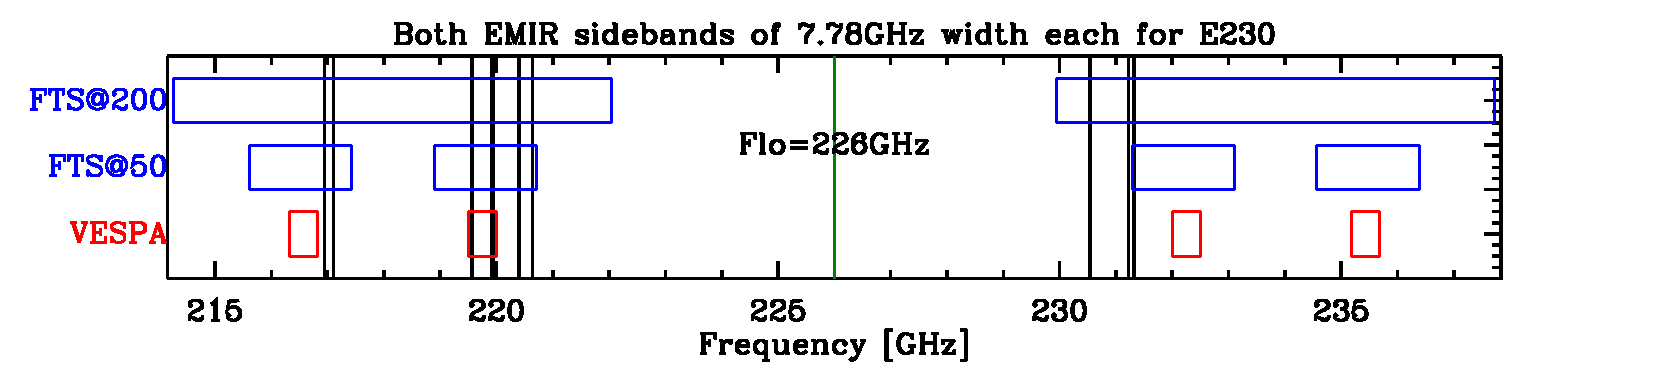
\includegraphics[width=0.8\textwidth]{figures/specsetup-1mm.pdf}
    \caption{Plages de fréquences sélectionnées pour les observations à \unmm.}
\end{figure}

\begin{figure}
    \centering
    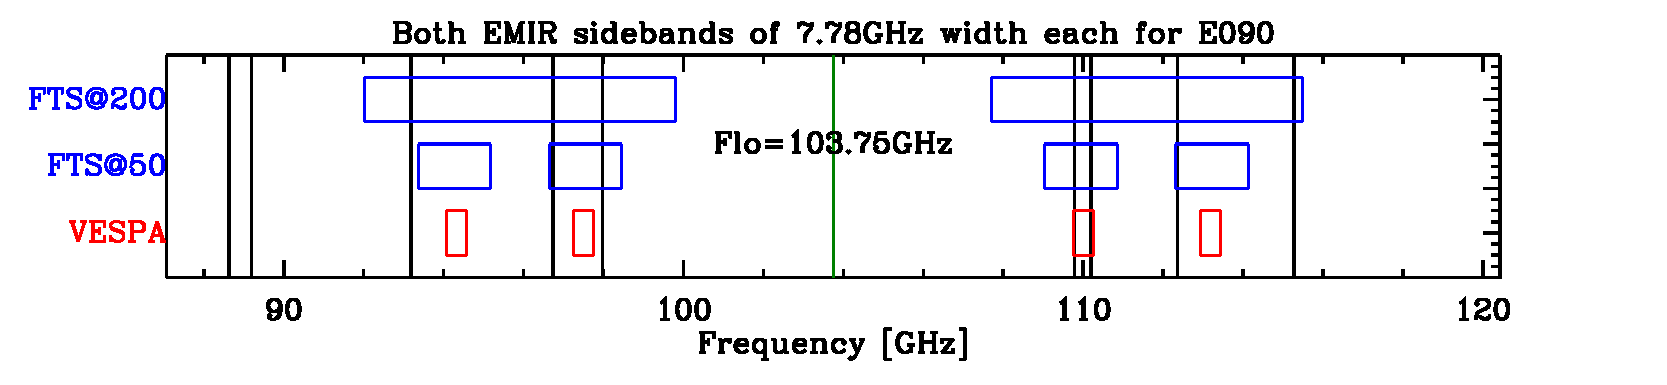
\includegraphics[width=0.8\textwidth]{figures/specsetup-3mm.pdf}
    \caption{Plages de fréquences sélectionnées pour les observations à \troismm.}
\end{figure}

\begin{figure}
    \centering
    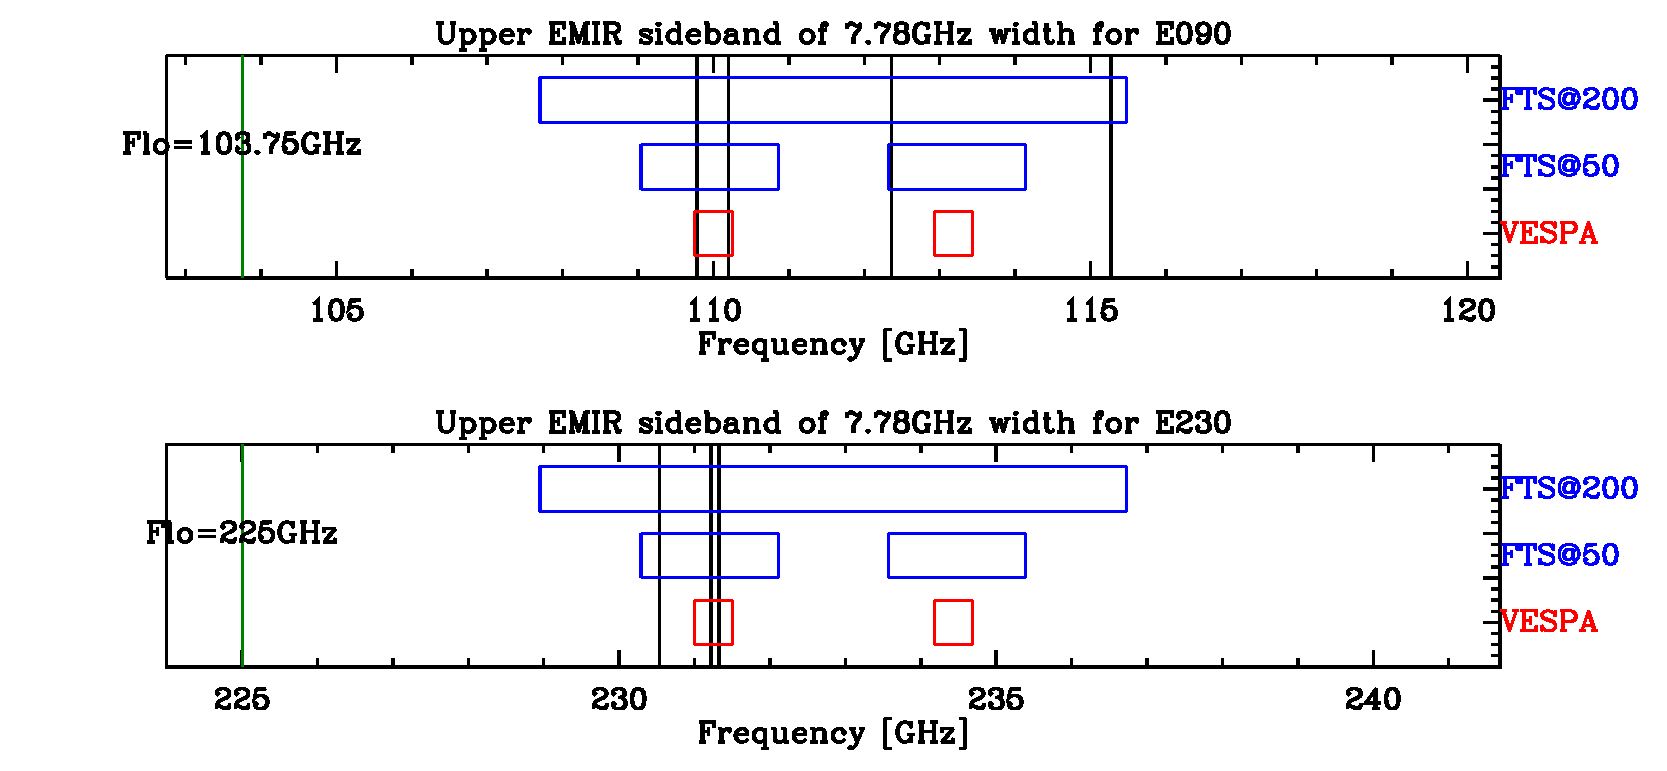
\includegraphics[width=0.8\textwidth]{figures/specsetup-3mm-1mm-u.pdf}
    \caption{Plages de fréquences sélectionnées pour les observations combinées à \unmm{} et \troismm.}
\end{figure}

\begin{figure}
    \centering
    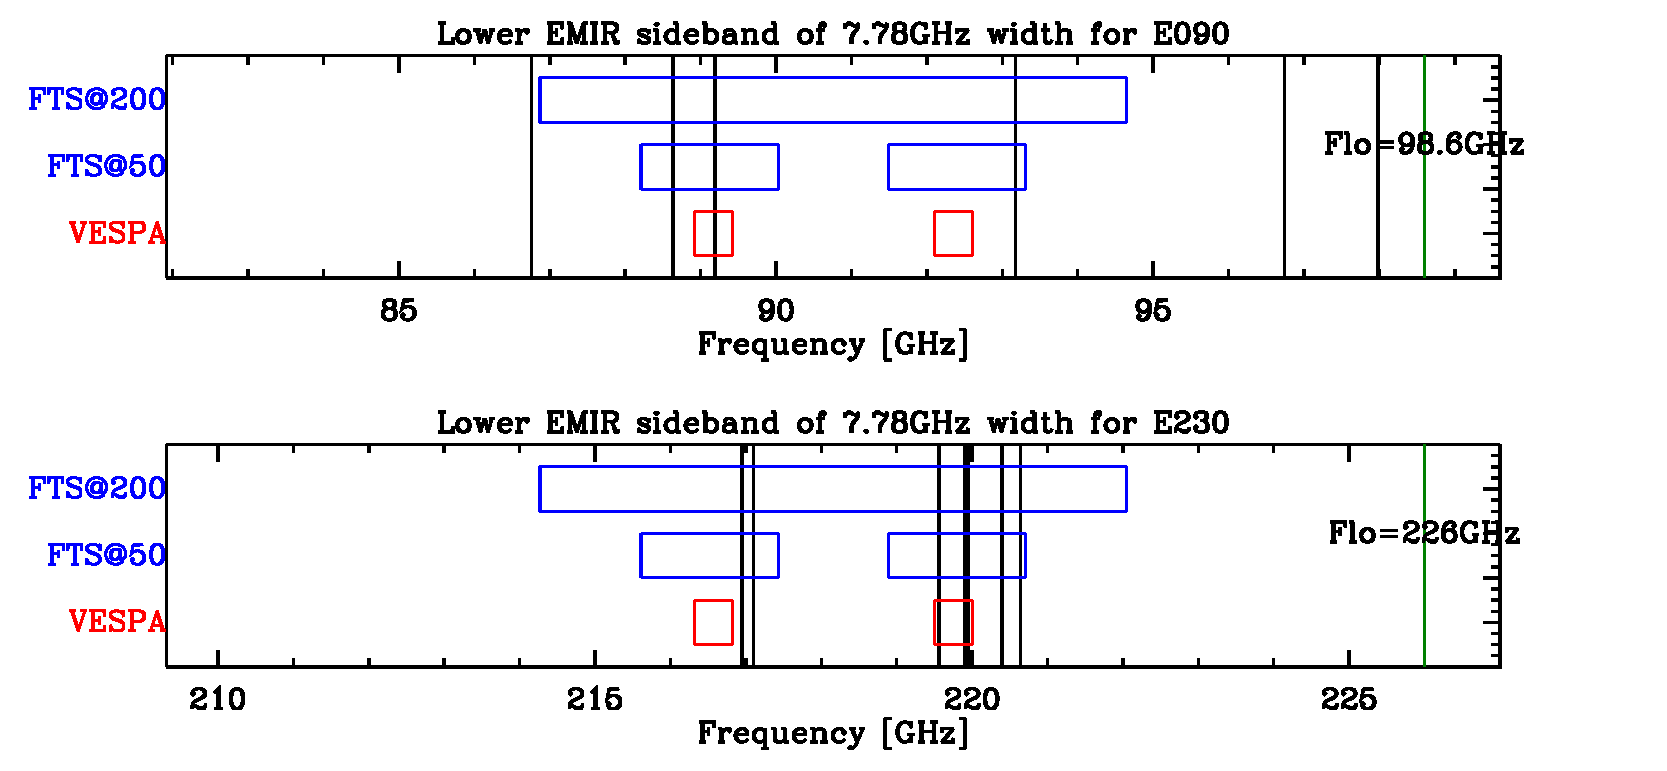
\includegraphics[width=0.8\textwidth]{figures/specsetup-3mm-1mm-l.pdf}
    \caption{Plages de fréquences complémentaires pour les observations combinées à \unmm{} et \troismm.}
\end{figure}

Sur place, la découverte du mode \textit{parallel} de VESPA grâce à la présence
de Gabriel \textsc{Paubert} en tant qu’\textit{Astronomer on duty} nous a
permis d’optimiser plus encore nos \textit{setups}.

\section{Le voyage}

TODO: Une petite photo ? Ou deux. :p Je vous laisse le choix, personellement j'ai pas ce qui faut pour ça (essentielement des nuages)

Le voyage a très bien organisé en amont. Les dates choisies pour le voyage
étaient parfaitement adaptées aux créneaux réservés pour nous au télescope (pas
de précipitation). Nous avons été très bien accueillis au télescope, autant par
les chercheurs présents que par le personnel de l’IRAM. Nous avons apprécié
tout particulièrement la présentation qui nous a été donnée le jour de notre
arrivée, ainsi que les échanges, fugaces mais riches, aux heures de repas. 

TODO: De Paris à Grenade via Madrid, visite de Grenade, de Grenade au Pico
Veleta en passant par l’arrêt à mi-hauteur.

Il est particulièrement agréable, arrivé en bas de la station, de doubler tous
les skieurs et autres surfeurs ainsi que l’ESF locale pour monter dans les
œufs. La partie du trajet effectuée en chenille donne un certain cachet à
l’expédition, même si beaucoup semblent nostalgiques de l’ancien véhicule, qui
donnait par son inconfort une véritable impression d’exploration aventurière.

Nous avons également pu profiter du premier jour sur place, sans observations,
pour nous promener un peu et faire quelques photos. Le lieu est vraiment
magnifique, et les paysages, dénués de touristes passé 17 h bien que le Soleil
soit encore relativement haut dans le ciel, splendides, particulièrement lors
du coucher de Soleil.

Nous avons également eu l’occasion de visiter l’intérieur du télescope en fin
de séjour, qui nous a permis de mieux appréhender l’instrumentation mise en
place et de réaliser la complexité de cette technologie, toujours fonctionnelle
après plus de 30 ans de loyaux services.

\section{Les observations}

TODO: Une photo de la salle de contrôle ? J’en ai quelques unes, avec ou sans nous (Bruno).

Le premier jour, nous avons commencé par prendre en main les différents outils
présents sur place : PaKo, Xephem, MIRA, TAPAS…

Les tâches étaient répartis sur 3 à 4 postes :
\begin{itemize}
    \item Un poste contrôlait Xephem pour vérifier le positionnement du
          télescope dans le ciel, pour contrôler sa position vis-à-vis du
          pointage demandé, vérifier sa position par rapport au Soleil, le
          choix de la topologie « high » ou « low » en fonction de la
          trajectoire des sources sur le ciel et des contraintes du télescope…
    \item Un second poste contrôlait PaKo pour gérer les instructions envoyées
          au télescope et vérifier la bonne prise en compte de celle-ci. C’est
          également à ce poste que le « cahier d’observations » TAPAS était
          rempli.
    \item Un troisième poste servait à analyser les données à l’aide de MIRA
          pour fournir les corrections à apporter dans PaKo et visualiser les
          résultats préliminaires.
    \item Un éventuel quatrième poste servait à traiter les données des jours
          précédents et celles s’ajoutant au fur et à mesure des observations
          pour en tirer les premiers résultats.
\end{itemize}

Toujours le premier jour, nous avons commencé dans un premier temps à nous
familiariser avec les différentes étapes à réaliser en début de chaque
observation :
\begin{itemize}
    \item Choix du \setup{} en fonction de la météo et des observations
          souhaitées, puis \textit{tuning} par l’opérateur. Nous remercions à
          cette occasion Manuel \textsc{Ruiz}, dit \textit{Manolo}, pour son incroyable
          efficacité ;
    \item Calibration puis \textit{pointing} sur une source de référence (ici,
          \textit{W3OH}), alternance de \textit{focus} et \textit{pointing} en
          fonction de leurs résultats respectifs ;
    \item Mesure (\textit{track}) sur une source de référence proche de la
          source observée pour obtenir un fond de carte ;
    \item Relevés sur la source proprement dite.
\end{itemize}

Nous observions chaque jour de 8 h 30 à 16 h. Le premier jour, nous avons
récupéré la main tôt : la météo fût catastrophique durant la nuit, et était
assez mitigée le matin. Nous avons donc décidé de commencer sur le \setup{} à
\troismm.

Comme c’était notre première session d’observation sur la source, il nous
fallait trouver une position de référence propre. En effet, l’un des problèmes
majeurs des observations à ces longueurs d’ondes est de trouver des zones
proches de la source sans émission, alors que \ce{^12CO} est une molécule
très abondante, particulièrement dans les nuages environnant les cœurs
pré-stellaires. En préparation, nous avions listé les coordonnées
d’emplacements potentiellement exempts d’émissions. Une fois les premières
étapes systématiques effectuées, nous avons donc effectué des relevés à chacune
des ces positions. À notre grand désespoir, aucune ne s’est avérée propre, et
elles étaient d’ailleurs toutes très similaires, pour une raison évidente
\textit{a posteriori} (\textit{cf.} \cref{sec:resultats}).

Le temps de réaliser tout ceci, la météo s’était fortement dégagée, mais
restait encore limite pour basculer à \unmm. Nous avons donc décidé d’être
partiellement conservateurs et de basculer sur le \setup{} intermédiaire
combinant \unmm{} et \troismm. Ainsi, si la météo se dégradait, nous aurions au
moins les données à \troismm{} d’exploitables. En pratique, le temps s’est
encore plus dégagé, pour aboutir à une opacité quasiment nulle. En fin de
journée, nous avons gardé un peu de temps pour persister dans nos recherches
d’une position de référence propre, toujours sans plus de succès.

Le second jour, la météo s’annonçait superbe dès le début : nous sommes partis
directement sur le \setup{} à \unmm. Enfin, presque. Nous avons eu quelques
soucis de fichiers de configuration manquants, heureusement rapidement
restaurés grâce à Gabriel.

Le troisième et dernier jour, la météo n’était pas très bonne. Nous avons
décidé d’utiliser uniquement le \setup{} à \troismm. Cependant, comme c’était
la première fois que nous utilisions ce \setup{} pour observer la source, nous
n’avions pas repéré une erreur présente dans le script \textit{OTF}. En effet,
l’\textit{offset} indiqué pour la position de référence était nul, car nous
devions le régler une fois cette position choisie. Ce que nous avions fait pour
l’autre script, mais pas celui-ci. Les premières données nous paraissaient
évidemment aberrantes, sans que nous ne comprenions pourquoi. Une fois de plus,
c’est l’arrivée de Gabriel, qui revenait du ski, qui nous a débloquée. Il a
tout suite suggéré de vérifier la position de référence, et nous nous sommes
aperçus de notre erreur. Heureusement, celle-ci était corrigible moyennant
quelques \textit{on/off} en \textit{frequency switching} avec la position de
référence et Anaëlle a réussi à réparer toutes les données.

Nous avons conclu cette dernière journée d’observations par une visite de
l’intérieur du télescope, très intéressante et instructive !

\section{Les données obtenues}
\label{sec:resultats}

Les résultats obtenus le premier jour ont été combinés avec ceux des jours
précédents, de sorte à obtenir des cartes plus précises. En effet, l’un des
intérêts de nos \textit{setups} était de pouvoir combiner facilement les
données issues des différentes observations.

TODO: Lister les raies observées, leurs caractéristiques et par conséquent la
présence d’outflow. Parler de la raie tellurique.

TODO: Fréquences bonus
HC3N(12-11)         109.1736

C17O(1-0)           112.359    J=1-0,     F=7/2-5/2
C17O(1-0)           112.360    J=1-0,     F=5/2-5/2

CN(1-0)             113.12337  J=1/2-1/2, F=1/2-1/2
CN(1-0)             113.14416  J=1/2-1/2, F=1/2-3/2
CN(1-0)             113.17049  J=1/2-1/2, F=3/2-1/2
CN(1-0)             113.19128  J=1/2-1/2, F=3/2-3/2
CN(1-0)             113.48812  J=3/2-1/2, F=3/2-1/2
CN(1-0)             113.49097  J=3/2-1/2, F=5/2-3/2
CN(1-0)             113.49964  J=3/2-1/2, F=1/2-1/2
CN(1-0)             113.50891  J=3/2-1/2, F=3/2-3/2
CN(1-0)             113.52043  J=3/2-1/2, F=1/2-3/2

TODO: Ajouter les figures de Jan.

\begin{figure}[h!]
\centering
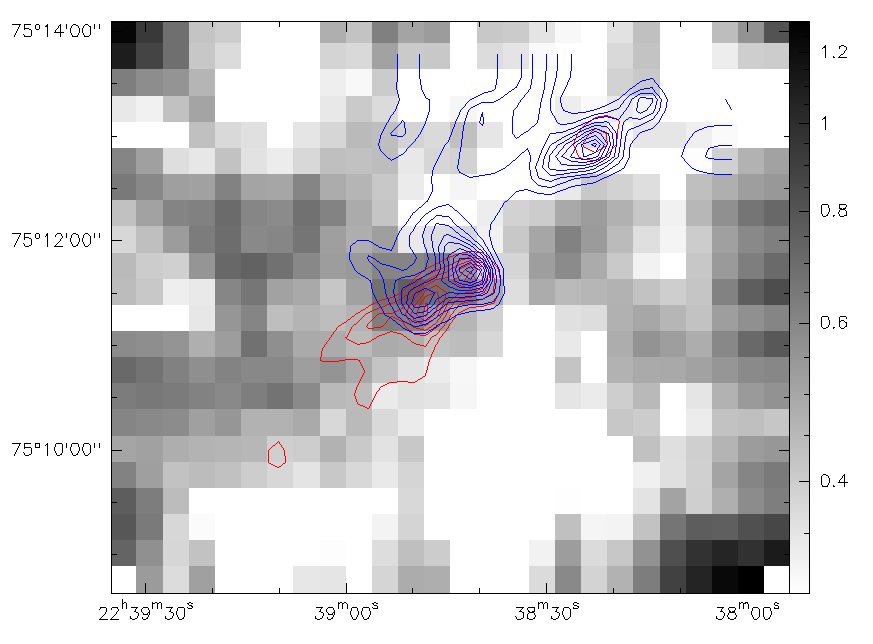
\includegraphics[height=6cm]{figures/mapC17O.png}
\caption{Carte des flots observés de CO. En bleu le $^{12}CO$ ``blueshifté'' En
    rouge le flot ``redshifté''. Les isocontours de vitesse sont pris avec
    comme réference la vitesse de la raie principale de $^{12}CO$ (2->1) à
    230.538 GHz, observée dans le \setup{} à \unmm. Les bins de densité ont été
    réalisés avec la raie de $^{17}CO$, meilleur traceur du gaz au repos.}
\label{mapC17O}
\end{figure}

\section*{Conclusion}
\addcontentsline{toc}{section}{Conclusion}

TODO: Visite de nuit, retour à Paris via Barcelone.

TODO: C’était cool et intéressant. On ajoute une autre photo.

Objectif du stage atteint : faire découvrir le fonctionnement, l'organisation d'un télescope. Bonne thématique scientifique.
Extrêmement enrichissant, surtout pour 4 étudiants plutôt branchés théorie. S'ils veulent convertir des gens à l'observation, il suffit de mettre en place ce stage en début d'année.

\end{document}
